\documentclass[10pt,aspectratio=169]{beamer}

\usetheme{Madrid}
\usecolortheme{default}
\usepackage[T1]{fontenc}
\usepackage{lmodern}
\usepackage{booktabs}
\usepackage{graphicx}
\usepackage{array}

\graphicspath{{../figs/}}

\title[Wheat Direction Forecasting]{Direction Forecasting on Daily U.S. Wheat Futures}
\subtitle{Leakage-safe ML evaluation and a preliminary long--flat overlay}
\author{Kenji Funaki}
\institute{NYU VIP Forecasting Project}
\date{May 2026}

\setbeamertemplate{navigation symbols}{}
\setbeamertemplate{footline}[frame number]

\begin{document}

\begin{frame}
  \titlepage
  \vspace{-1.5ex}
  \begin{block}{Project objective}
  Forecast next-day wheat direction using public daily prices, macro data, and machine learning, then test whether predicted probabilities can support a modest tactical long--flat rule.
  \end{block}
\end{frame}

\begin{frame}{Data Pipeline and Leakage Controls}
  \begin{columns}[T,onlytextwidth]
    \begin{column}{0.52\textwidth}
      \begin{itemize}
        \item Daily Chicago SRW wheat futures plus engineered technical features.
        \item FRED-MD macro indicators transformed by stationarity codes and shifted by one month.
        \item Optional cross-asset returns: corn, soybeans, UUP, and CAD.
        \item Chronological split: train/CV first, final 15\% holdout last.
        \item Scalers and PCA fit only on training folds or train+validation rows.
      \end{itemize}
    \end{column}
    \begin{column}{0.45\textwidth}
      \centering
      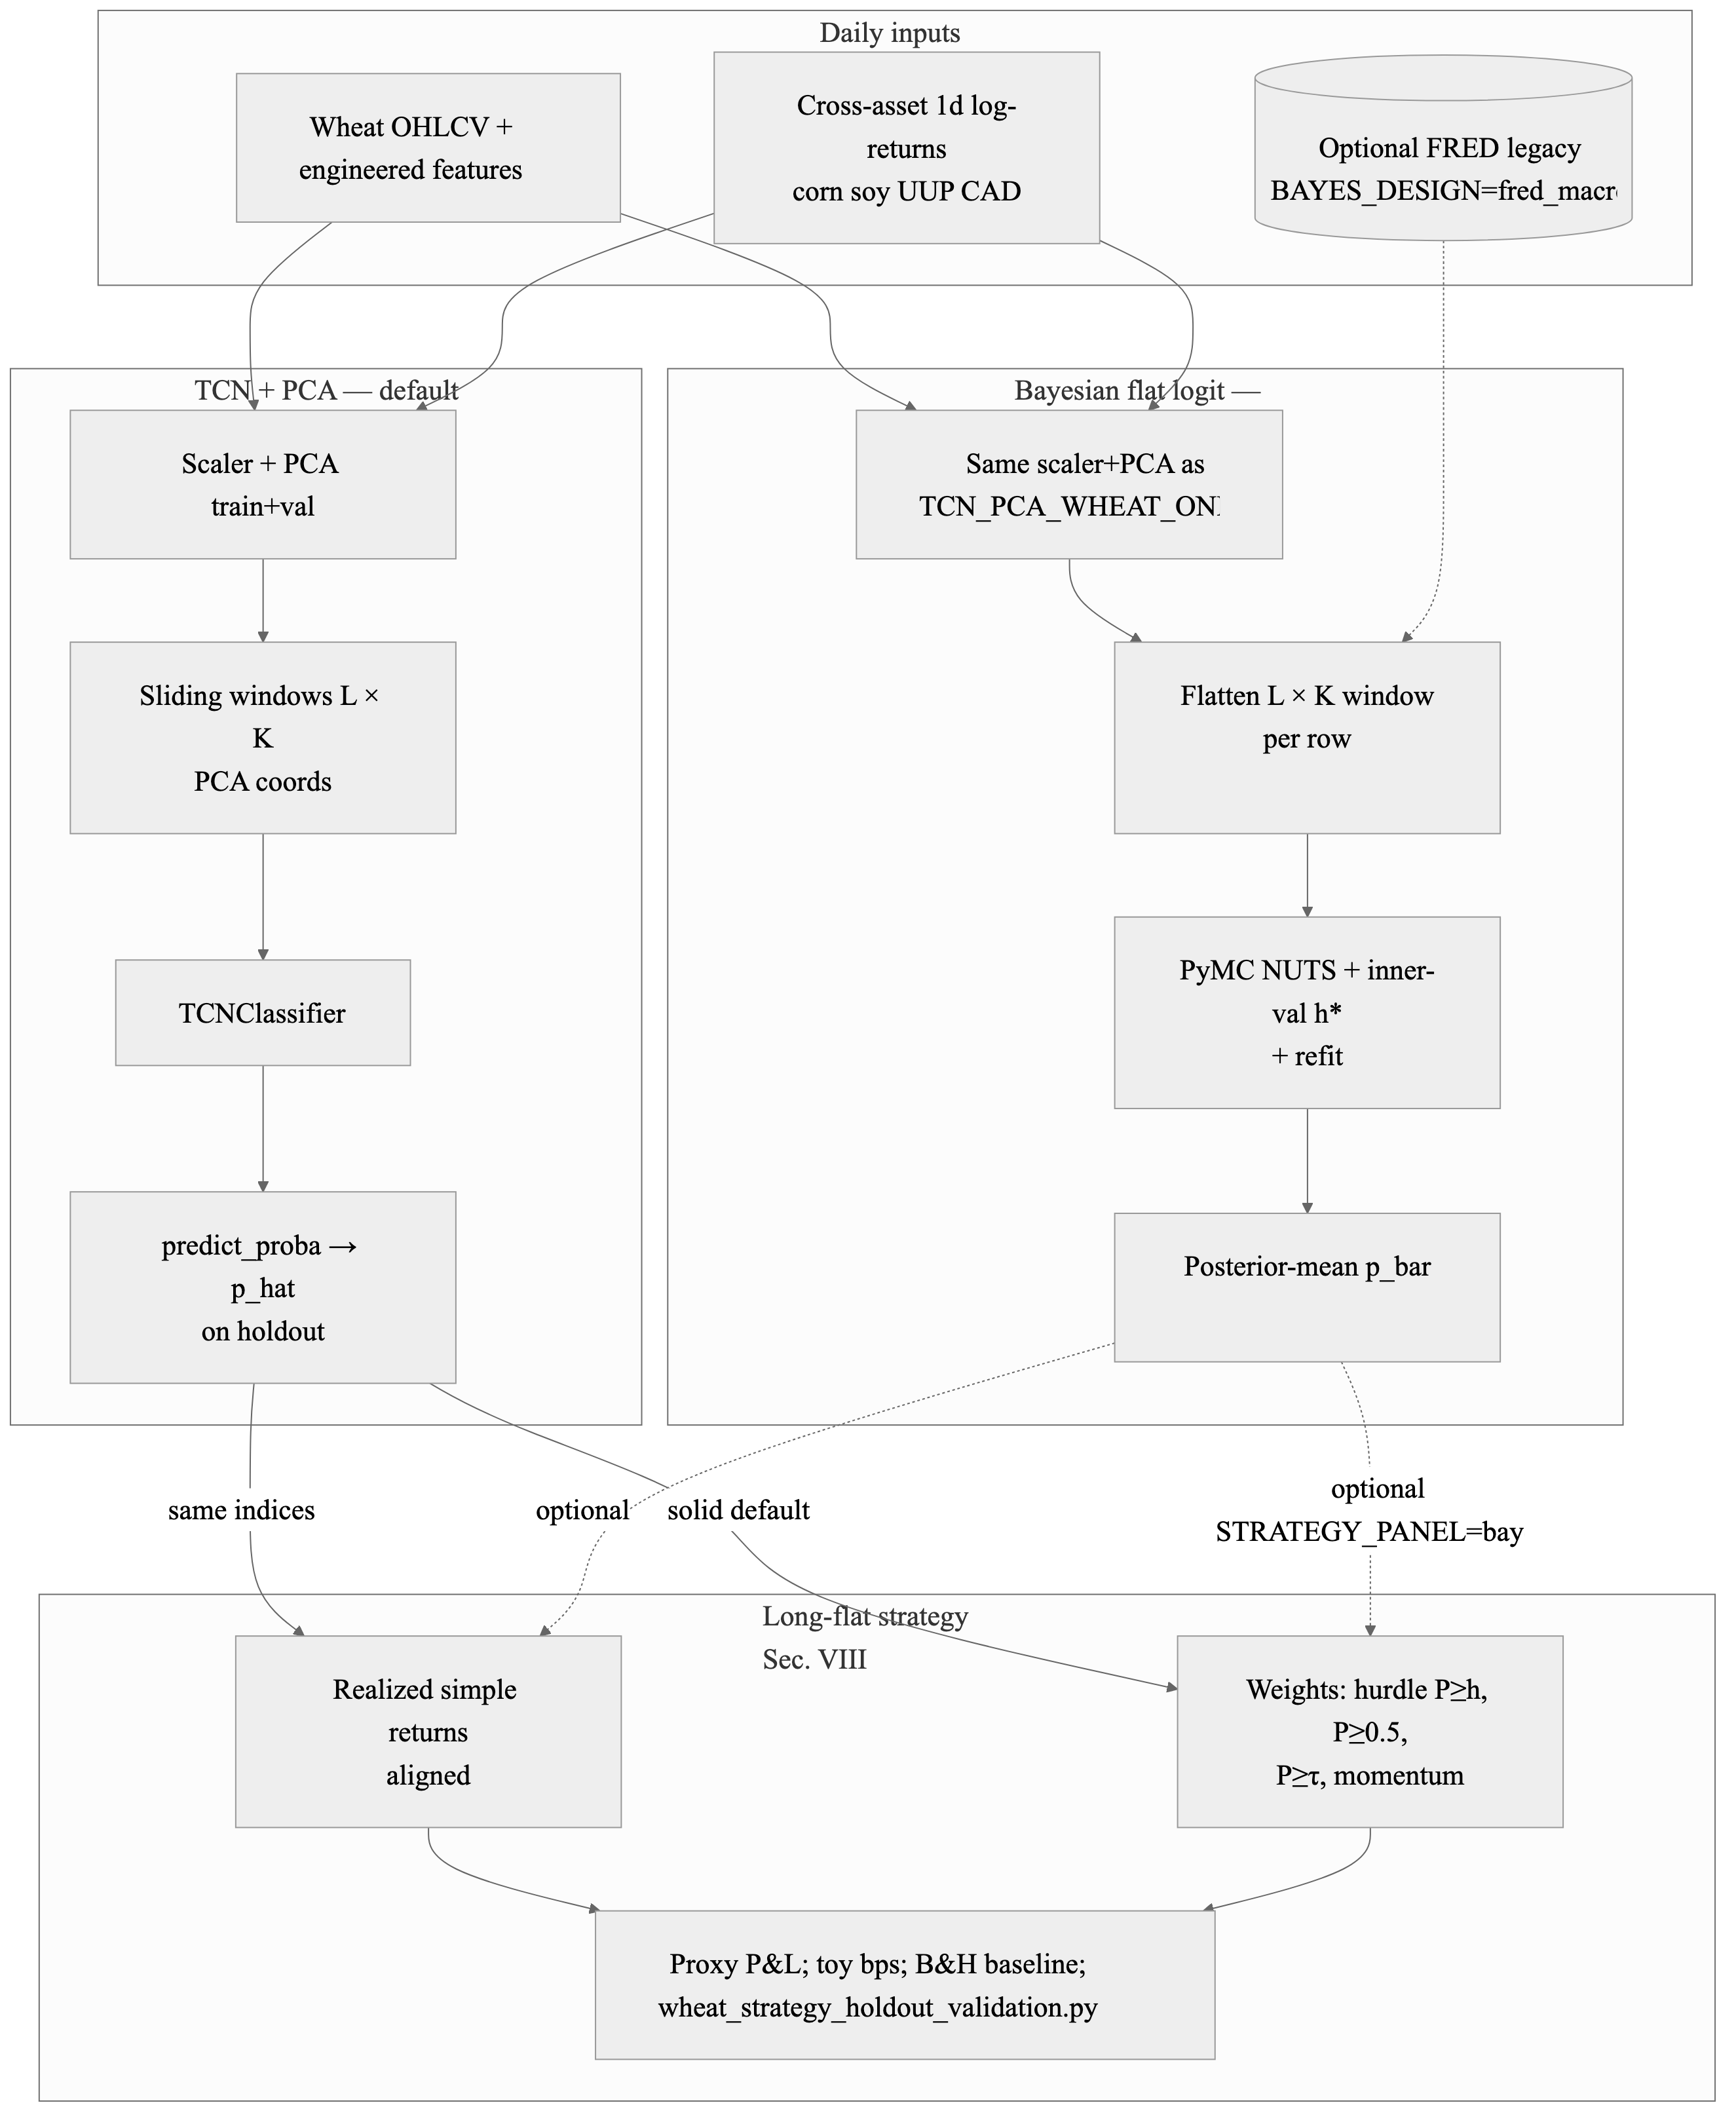
\includegraphics[width=\linewidth,height=0.72\textheight,keepaspectratio]{pipeline_tcn_pca_mcmc_strategy.png}
    \end{column}
  \end{columns}
\end{frame}

\begin{frame}{Models and Main Forecasting Results}
  \small
  \begin{table}
    \centering
    \begin{tabular}{@{}lccc@{}}
      \toprule
      Model & Holdout Acc. & ROC-AUC & Macro F1 \\
      \midrule
      FAVAR & 0.514 & 0.508 & 0.513 \\
      ARX   & 0.523 & 0.526 & 0.522 \\
      ELM   & 0.512 & \textbf{0.528} & 0.511 \\
      TCN   & \textbf{0.541} & 0.526 & \textbf{0.541} \\
      \bottomrule
    \end{tabular}
  \end{table}
  \begin{itemize}
    \item TCN was the best classifier on the terminal holdout, but fold scores stayed close to 0.50.
    \item Reported differences are descriptive, not statistically significant superiority claims.
    \item Main lesson: forecasting wheat direction is hard; leakage-safe evaluation matters more than headline accuracy.
  \end{itemize}
\end{frame}

\begin{frame}{Most Recent Work: Probabilities to a Long--Flat Overlay}
  \small
  \begin{columns}[T,onlytextwidth]
    \begin{column}{0.52\textwidth}
      \begin{itemize}
        \item Use TCN probability \(\hat p_t\) to decide when to be long versus flat.
        \item Compare buy-and-hold, fixed probability hurdles, validation threshold \(\tau\), and momentum.
        \item Bayesian logistic MCMC adds posterior-mean probabilities \(\bar p_t\) for uncertainty-aware variants.
        \item This is a frictionless proxy: no commissions, rolls, margin, options, or live execution assumptions.
      \end{itemize}
    \end{column}
    \begin{column}{0.45\textwidth}
      \centering
      \begin{tabular}{@{}lrr@{}}
        \toprule
        Rule & Total ret. & \% long \\
        \midrule
        Buy-and-hold & -0.468 & 1.00 \\
        \(p\ge0.52\) & 0.000 & 0.00 \\
        \(p\ge0.50\) & 0.009 & 0.001 \\
        \(p\ge\tau\) & 0.000 & 0.42 \\
        Momentum & -0.155 & 0.46 \\
        \bottomrule
      \end{tabular}
      \vspace{1ex}

      \footnotesize One bearish holdout tail: risk exposure mattered more than tiny accuracy gaps.
    \end{column}
  \end{columns}
\end{frame}

\begin{frame}{Lessons Learned and What I Would Add}
  \begin{itemize}
    \item Leakage prevention is the core engineering challenge: chronological splits, fold-safe scaling, and lagged macro releases are non-negotiable.
    \item Alternative data and PCA helped organize features, but signal remains modest and unstable across slices.
    \item Nonlinear models can edge transparent baselines, but probability calibration and uncertainty are more useful than overclaiming alpha.
    \item A realistic next step is an expanding-window walk-forward test with nested tuning, FRED-vintage sensitivity, costs, and roll logic.
    \item Presentation takeaway: this is a reproducible empirical evaluation study, not an ``AI trading system.''
  \end{itemize}
\end{frame}

\end{document}
